% Declare type of document
\documentclass[10pt]{article}

% Import Packages
\usepackage[utf8]{inputenc}

% Commonly used math symbols and fonts
\usepackage[mathscr]{euscript}
\usepackage{amsfonts,amsmath,amssymb,amsthm}
\usepackage{mathtools,mathdots}

% Better looking default font
\usepackage{lmodern}

% itemize environment
\usepackage{enumitem}

% Array, longtable, and booktabs
\usepackage{array}
\usepackage{longtable}
\usepackage{booktabs}

% Caption package for hiding Figure #
\usepackage{caption}

% Page formatting
\usepackage[letterpaper, margin=1in]{geometry}

% Package for nice syntax highlighting for code
\usepackage{minted}

% Allows line breaks in the math environment
\allowdisplaybreaks

\usepackage[activate={true,nocompatibility},final,tracking=true,kerning=true,spacing=true,factor=1100,stretch=10,shrink=10]{microtype}
\microtypecontext{spacing=nonfrench}
% activate={true,nocompatibility} - activate protrusion and expansion
% final - enable microtype; use "draft" to disable
% tracking=true, kerning=true, spacing=true - activate these techniques
% factor=1100 - add 10% to the protrusion amount (default is 1000)
% stretch=10, shrink=10 - reduce stretchability/shrinkability (default is 20/20)


\title{CS 310: Linked List}
\author{Connor Baker}
\date{January 31, 2019}

\begin{document}

\maketitle

\subsection*{List}
\begin{itemize}
    \item List notation from JavaDoc
    \begin{itemize}
        \item package \mintinline{java}{java.util};
        \item \mintinline{java}{public interface List<E> extends Collection<E>}
        \item An \textbf{unordered} collection (also known as a \textbf{sequence}). The user of this interface has precise control over where in the list each element is inserted. The user can access elements by their integer index (position in the list), and search for elements in the list.
        \item Basic operations: \mintinline{java}{.get()}, \mintinline{java}{.set()}, \mintinline{java}{.add()}, \mintinline{java}{.remove()} 
    \end{itemize}
    \item Implementation
    \begin{itemize}
        \item Dynamic array: based on contiguous memory
        \item Linked lists: based on a series of linked nodes residing in (typically non-contiguous) memory
    \end{itemize}
\end{itemize}

\subsection*{Singly-Linked List}
\begin{center}
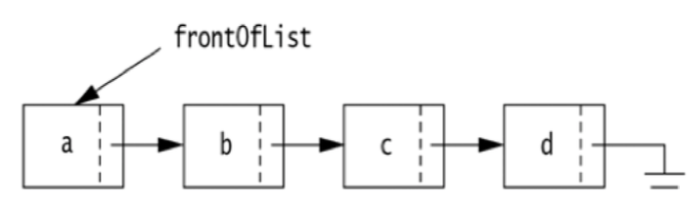
\includegraphics[width=\textwidth/4]{images/1.png}
\end{center}
\begin{itemize}
    \item Weiss Figure 17.1
    \item Node structure
    \begin{itemize}
        \item How do we define the link between nodes?
    \end{itemize}
    \item We can make a node that is a reference to an object, or we can make a truly generic node
    \begin{itemize}
        \item The \mintinline{java}{Object} variety:
        \begin{minted}{java}
class ListNode {
    Object element;
    ListNode next;
}
        \end{minted}
        \item The generic variety:
        \begin{minted}{java}
class ListNode<T> {
    T value;
    ListNode<T> next;
}
        \end{minted}
    \end{itemize}
\end{itemize}

\subsection*{Linked List: Insertion}
\begin{center}
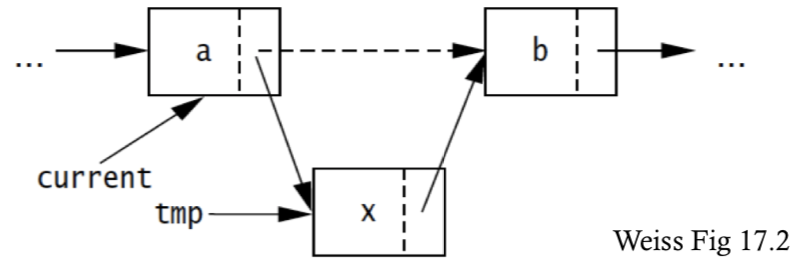
\includegraphics[width=\textwidth/4]{images/2.png}
\end{center}
\begin{itemize}
    \item Create a new node
    \item Set the fields of the new node: \mintinline{java}{data(value)}, \mintinline{java}{next}
    \item Add the node into the linked list
    \begin{itemize}
        \item Find the point to insert; set/update links
    \end{itemize}
    \item \textit{No need to shift elements!}
\end{itemize}

\subsection*{Linked List: Deletion}
\begin{center}
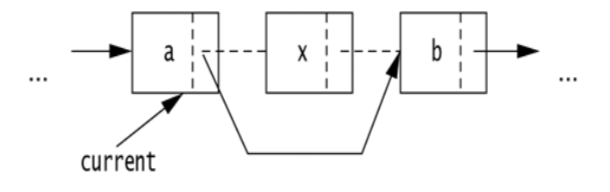
\includegraphics[width=\textwidth/4]{images/3.png}
\end{center}
\begin{itemize}
    \item Set the \mintinline{java}{next} of the old predecessor
    \item What do we do with \mintinline{java}{Node x}?
    \begin{itemize}
        \item Just un-link it from the other nodes. Without a reference to it, the node is garbage collected.
    \end{itemize}
    \item What do we do if we want to delete the first node?
    \begin{itemize}
        \item Just shift the head to the next item.
    \end{itemize}
    \item \textit{No need to shift elements!}
\end{itemize}

\subsection*{Demo}
\begin{center}
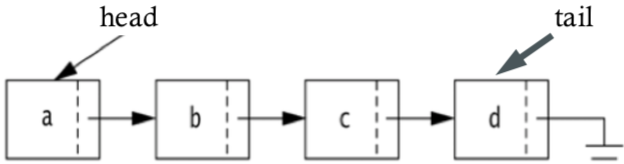
\includegraphics[width=\textwidth/4]{images/4.png}
\end{center}
\begin{itemize}
    \item Singly-linked list to implement a list type
    \begin{itemize}
        \item Internally maintain a linked list
        \begin{itemize}
            \item Node type
            \item Special reference to \mintinline{java}{head}/\mintinline{java}{tail}
        \end{itemize}
        \item Externally support the same operations: \mintinline{java}{.get()}, \mintinline{java}{.set()} (or \mintinline{java}{.replace()}), \mintinline{java}{.append()}, \mintinline{java}{.insert()}, \mintinline{java}{.remove()}, \mintinline{java}{.indexOf()}...
    \end{itemize}
\end{itemize}

\subsection*{Create \mintinline{java}{MyList}}
\begin{minted}{java}
public class MyLList<T> {
    ...
    public int size(); // Number of items stored
    public void append(T x); // Add an element to the end of the list
    public T get(int i); // Access the i-th element
    public void set(int i, T x); // Can only replace existing elements
    public void insert(int i, T x); // Insert at position i
    public T remove(int i); // Remove element at position i
    public int indexOf(T x);
}
\end{minted}

\subsection*{Operations on Lists}
\begin{center}
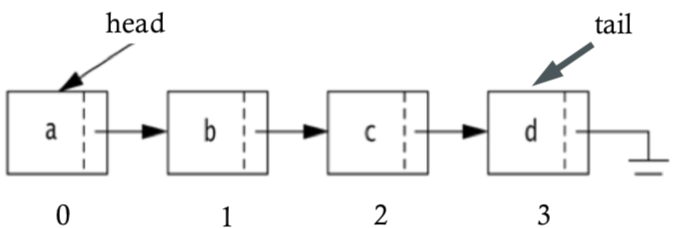
\includegraphics[width=\textwidth/4]{images/5.png}
\end{center}
\begin{itemize}
    \item Define an internal index based on the location with respect to the head of the linked list
    \begin{itemize}
        \item \mintinline{java}{.set(i, x)} and \mintinline{java}{.get(i)}
    \end{itemize}
    \item Changing the membership
    \begin{itemize}
        \item \mintinline{java}{.append(x)}: insert at the tail (which updates where the tail is pointing)
        \item \mintinline{java}{.insert(i, x)}, \mintinline{java}{.remove(i, x)}: link in a new node or de-link a node
    \end{itemize}
    \item Iteration
    \begin{itemize}
        \item \mintinline{java}{.indexOf(x)}, \mintinline{java}{.contains(x)}
        \item \mintinline{java}{Iterator}: discuss later
    \end{itemize}
\end{itemize}

\subsection*{Implementation}
\begin{itemize}
    \item Demo
\end{itemize}

\subsection*{Key Observations}
\begin{itemize}
    \item No pre-defined index like static/dynamic array
    \begin{itemize}
        \item More expensive operations involving an index
    \end{itemize}
    \item Most of the time we'll need to traverse the linked list
    \begin{itemize}
        \item To traverse: how do we know where to start and where to stop?
        \item For every node: what do we do with the current node? How do we know there is another node? How do we get to the next node, if it exists?
    \end{itemize}
\end{itemize}

\subsection*{Complexity}
\begin{itemize}
    \item Linked list of size $N$
    \begin{center}
    \begin{tabular}{l>{$}r<{$}}\toprule
        Method & \text{Big-}O \\ \midrule
        \mintinline{java}{.size()} & O(1) \\
        \mintinline{java}{.get(i)} & O(n) \\
        \mintinline{java}{.set(i, x)} & O(n) \\
        \mintinline{java}{.append(x)} & O(1) \\
        \mintinline{java}{.insert(i, x)} & O(n) \\
        \mintinline{java}{.remove(x)} & O(n) \\
        \mintinline{java}{.contains(x)} & O(n) \\ \bottomrule
    \end{tabular}
    \end{center}
    \item How's the space complexity?
    \begin{itemize}
        \item Not great -- for each node, we must maintain a reference to the next node. It's $O(2n)$ (assuming that a reference to a node is the same size as a reference to the datum), which is $O(n)$, but still.
    \end{itemize}
\end{itemize}

\subsection*{Linked List Variants}
\begin{itemize}
    \item List fields
    \begin{itemize}
        \item Keep a reference to \mintinline{java}{head} node
        \item Keep a reference to \mintinline{java}{tail} node
        \item Use a dummy header node
    \end{itemize}
    \item Node fields
    \begin{itemize}
        \item Reference to the next node (\textbf{singly}-linked list)
        \item Reference to both previous and next nodes (\textbf{doubly}-linked list)
    \end{itemize}
\end{itemize}

\subsection*{Header Node}
\begin{itemize}
    \item Now we can remove the node from any location consistently
    \item Non-empty linked list:
    
    \begin{center}
        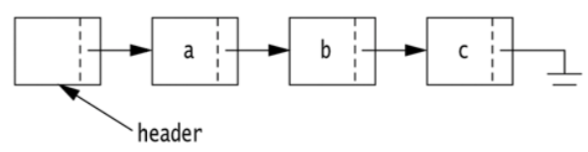
\includegraphics[width=\textwidth/4]{images/6.png}
    \end{center}
    
    \item Or an empty list with only a header:
    
    \begin{center}
        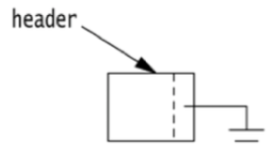
\includegraphics[width=\textwidth/8]{images/7.png}
    \end{center}
\end{itemize}

\subsection*{Doubly Linked List}
\begin{center}
    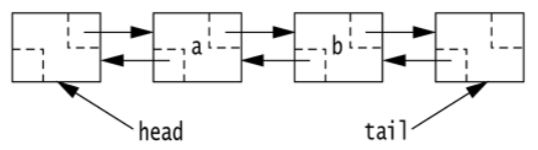
\includegraphics[width=\textwidth/4]{images/8.png}
\end{center}

\subsection*{Doubly Linked List: Insertion}
\begin{center}
    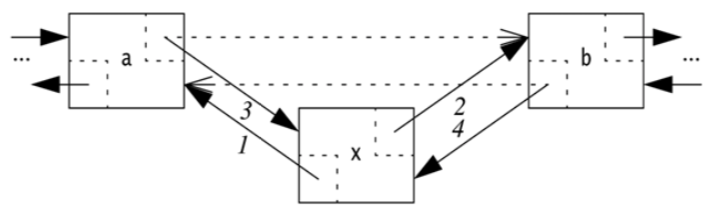
\includegraphics[width=\textwidth/4]{images/9.png}
\end{center}
\begin{itemize}
    \item Be careful about the order
\end{itemize}

\subsection*{Linked List Comparison}
\begin{center}
\begin{tabular}{lllllll}\toprule
    Implementation & get/set & add/del at end & add/del at start & add/del at mid & search & can grow? \\ \midrule
        Singly-Linked & $N$ & 1, $N$ & 1 & $N$ & $N$ & yes \\
        Doubly-Linked & $N$ & 1 & 1 & $N$ & $N$ & yes \\ \bottomrule
\end{tabular}
\end{center}
\begin{itemize}
    \item Singly linked list \mintinline{java}{.add()}is constant time but \mintinline{java}{.remove()} requires searching down to the node before the end to set it to null
    \item Remember: to insert and remove from the middle you first have to search for the correct position in the list, which is $O(n)$
    \item Doubly linked uses more memory, but is still $O(n)$
\end{itemize}

\subsection*{Array vs. Linked List}
\begin{itemize}
    \item Array/Static array -- a ``row" of memory
    \begin{itemize}
        \item We can run out of space with these because they are static
    \end{itemize}
    \item Dynamic arrays -- arrays that can grow in size
    \begin{itemize}
        \item Cost to copy repeatedly (not so bad)
        \item Insert/remove is expensive (one of the worst performance aspects)
    \end{itemize}
    \item Linked Lists -- tiny blocks of memory ``linked" together
    \begin{itemize}
        \item No ``quick" memory access since we must traverse an array
        \item Bad space complexity -- there's a lot of memory wasted on just keeping track of addresses
    \end{itemize}
\end{itemize}

\subsection*{Arrays vs. Others}
\begin{itemize}
    \item Arrays are simple
    \begin{itemize}
        \item \mintinline{java}{.get()} and \mintinline{java}{.set()} are trivial
        \item \mintinline{java}{.add()} and \mintinline{java}{.remove()} are obvious (though we need to keep track of the size of the structure)
        \item Very clear how data is laid out (it is contiguous, after all)
    \end{itemize}
    \item Just about every other data structure is more complicated
    \begin{itemize}
        \item \mintinline{java}{.get()} and \mintinline{java}{.set()} are nontrivial
        \item We have to preserve some internal structure so that we can control access
        \item Element-by-element access takes time
    \end{itemize}
\end{itemize}

\subsection*{List Implementation $\mathbf{O(n)}$ Summary}
\begin{center}
    \begin{tabular}{lcccccr} \toprule
        Implementation & get/set & add/del at end & add/del start & add/del mid & search & can grow? \\ \midrule
        Static Array & 1 & 1 & $N$ & $N$ & $N$ & no \\
        Dynamic Array & 1 & $\mathbf{1^*}$ & $N$ & $N$ & $N$ & no \\     Singly-Linked & $N$ & 1, $N$ & 1 & $N$ & $N$ & yes \\
        Doubly-Linked & $N$ & 1 & 1 & $N$ & $N$ & yes \\ \bottomrule
    \end{tabular}
    \begin{center}*Amortized analysis\end{center}
\end{center}

\subsection*{Extra: Sorting with Linked List}
\begin{itemize}
    \item How do we do the following with a linked list?
    \begin{itemize}
        \item Insertion
        \begin{itemize}
            \item Insert using a \mintinline{java}{Comparator} to insert after the greatest lower bound.
        \end{itemize}
        \item Selection
        \item Big-O?
        \begin{itemize}
            \item It'll be $O(n)$ since we're effectively searching through the entire list before inserting our object.
        \end{itemize}
    \end{itemize}
    
    \item How do we code with a linked list?
    \begin{itemize}
        \item Could you implement \mintinline{java}{.orderedInsert(x)}?
        \item Could you implement \mintinline{java}{.selectionSort(x)}?
    \end{itemize}
\end{itemize}

\subsection*{Summary}
\begin{itemize}
    \item Linked list
    \begin{itemize}
        \item Basic structure; insertion/deletion/search
        \item There are a number of variations
        \item Practice by completing the code, adding more methods, and try variations
        \begin{itemize}
            \item Doubly-linked lists, list with header nodes, etc...
            \item \mintinline{java}{.orderedInsert(x)}, \mintinline{java}{.clear()}, etc...
        \end{itemize}
        \item Time/space analysis
    \end{itemize}
    \item Next lecture: \mintinline{java}{Iterator}
    \begin{itemize}
        \item Reading: Chapter 6, Chapter 15
    \end{itemize}
\end{itemize}


\end{document}